\section{Konstrukce dvířek}\label{sec:konstrukce-dvirek}
Elektrická dvířka systému Coopmaster jsou tím hlavním důvodem proč tento projekt vůbec vznikl.
Prozatím se jedná o prototyp vlastní konstrukce, který se bude před trvalou instalací ještě zdokonalen a konstrukce bude navržena vzhledem k ceně řešení a na míru potřebám chovatele.
Aktuálně jsou dvířka sestavena ze standardních hliníkových profilů.
Pro pohyb dvířek se pro prototyp jeví jako nejsnažší volba táhlový motor na napětí 12V stejnosměrných (popis v sekci~\ref{sec:tahlovy-motor}).
Tento motor je připevněn ke kovovému plátu, který slouží jako posuvná dvířka.
Důležité je motor propojit s dvířky nějakým flexibilním spojem.
Já ve svém řešení použil obyčejný provázek.
Pokud by byl totiž plát připevněn pevně k motoru, mohla by se snadno stát nepřijemná situace, kdy by v případě zaseknutí slepice v prostoru dvířek během zavírání mohlo dojít k jejímu rozpůlení, což samozřejmě není žádoucí.
Řešení má také svou slabou stránku v nedostatečném výsuvu motoru, kvůli kterému bylo potřeba použít kladku ke zdvojnásobení výsuvu, aby slepice vůbec prolezla pod plátem.
Ačkoli má toto řešení řadu nevýhod a konstrukčních vad, tak bylo realizováno jednoduše z toho důvodu, že jsem většinu součástek měl doma již z minulých projektů.
I kdyby se do budoucna vyřešili zmíňované problémy řešení by pořád nebylo produkční, protože hliníkové součásti společně s motorem jsou příliš drahé a je zbytečné si do kurníku instalovat dvířka, která svou cenou převýší cenu vajec, které vyprodukujete za rok.
Nicméně náš projekt je aktuálně ve fázi vývoje, kdy řešíme spíše softwarovou než hardwarovou stránku, takže jsou pro testovací účeli aktuální dvířeka vyhovující díky možnosti snadných úprav a ladění konstukce.
Na obrázku~\ref{fig:proto_dvirka} můžete vidět aktuální podobu dvířek instalovaných u kurníku.

\begin{figure}[h]
    \centering
    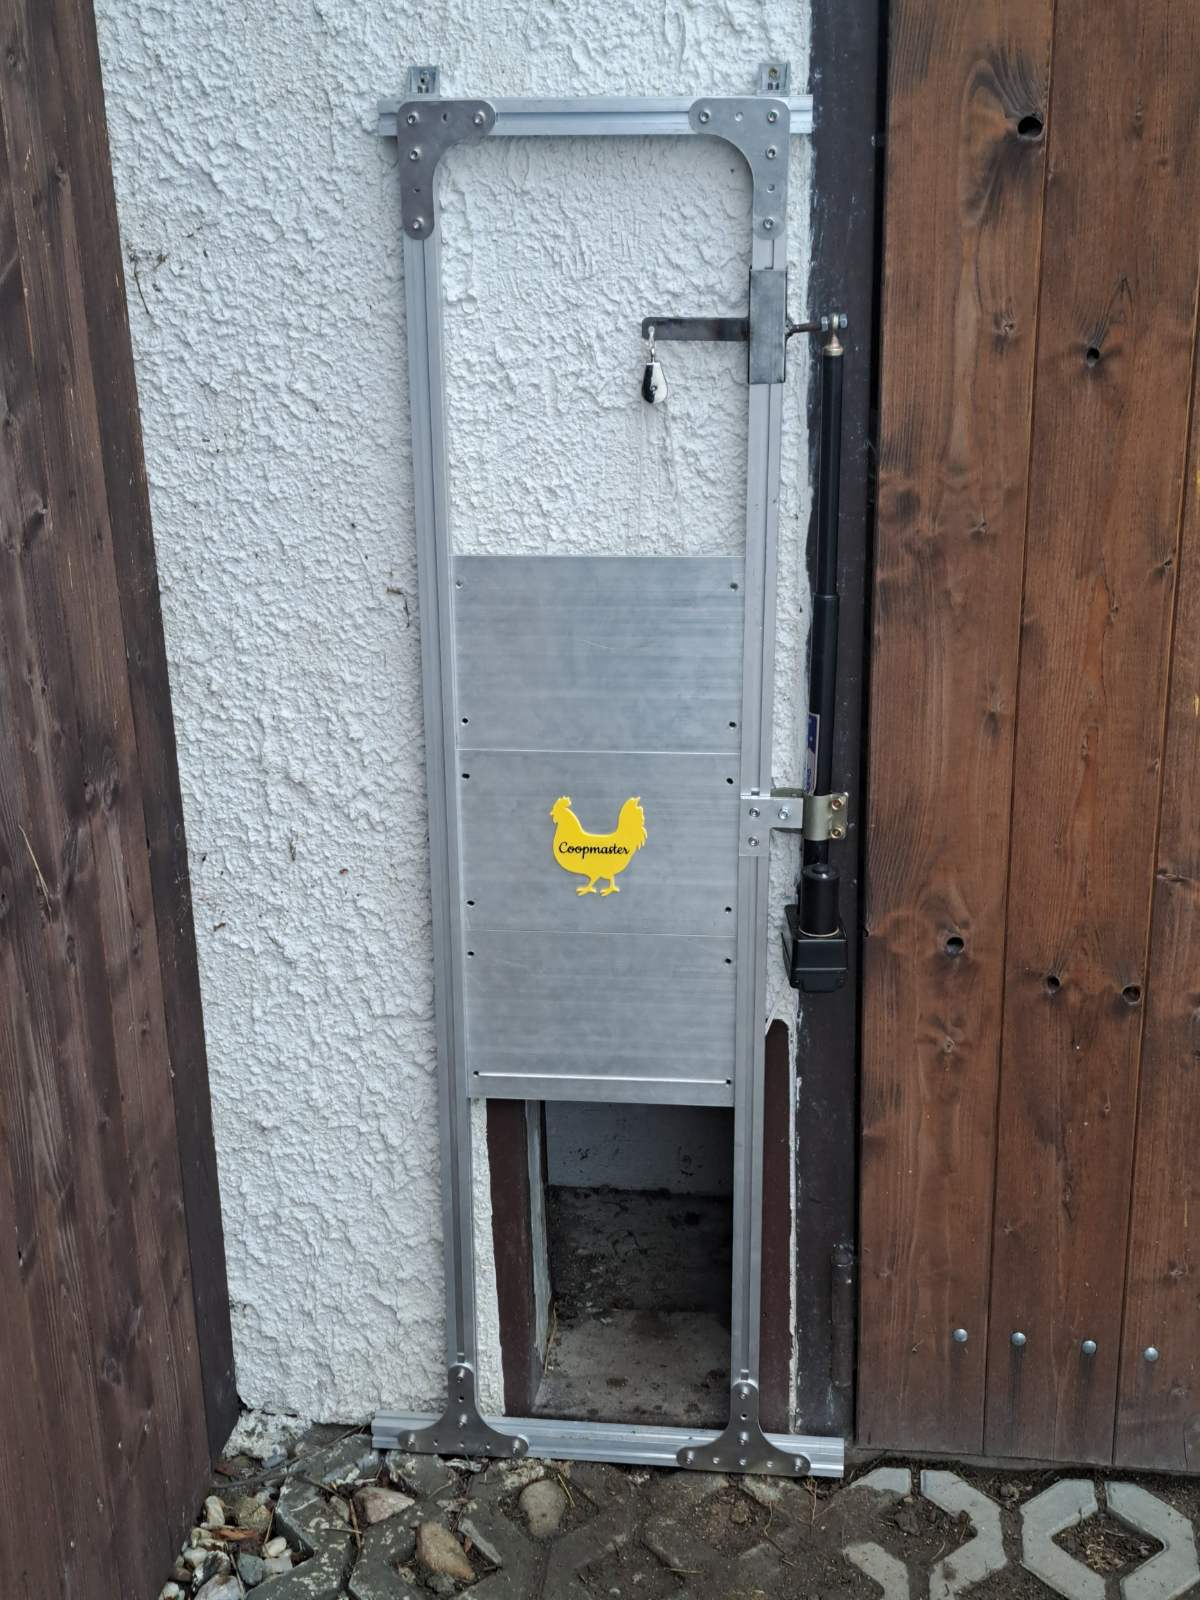
\includegraphics[width=\textwidth]{img/proto_dvirka}
    \caption{Instalovaný prototyp dvířek}
    \label{fig:proto_dvirka}
\end{figure}

%konstrukce dveri - expoziční
%- přímočarý motor s dorazy
%- konstrukce z hliníkových profilů a smontnotváno pomocí běžných spojovacích prvků pro práci s těmito profily
%- dvířka reprezentována hliníkovým plátem tahaným lankem připěvněným k ramenu který vynáší sílu od motoru k dvířkům
%- zdroj 12V
